\section{Theory}

\subsection{Haplogroups}

The human Y chromosome is only inherited from father to
son. Usually large parts of it are unchanged but sometimes
a mutation at a single position occurs. Such mutations are
called SNPs (Single Nucleotide Polymorphisms). They are
very stable and can be used to group people into ancestral
lines.

\begin{figure}[ht]
\centering
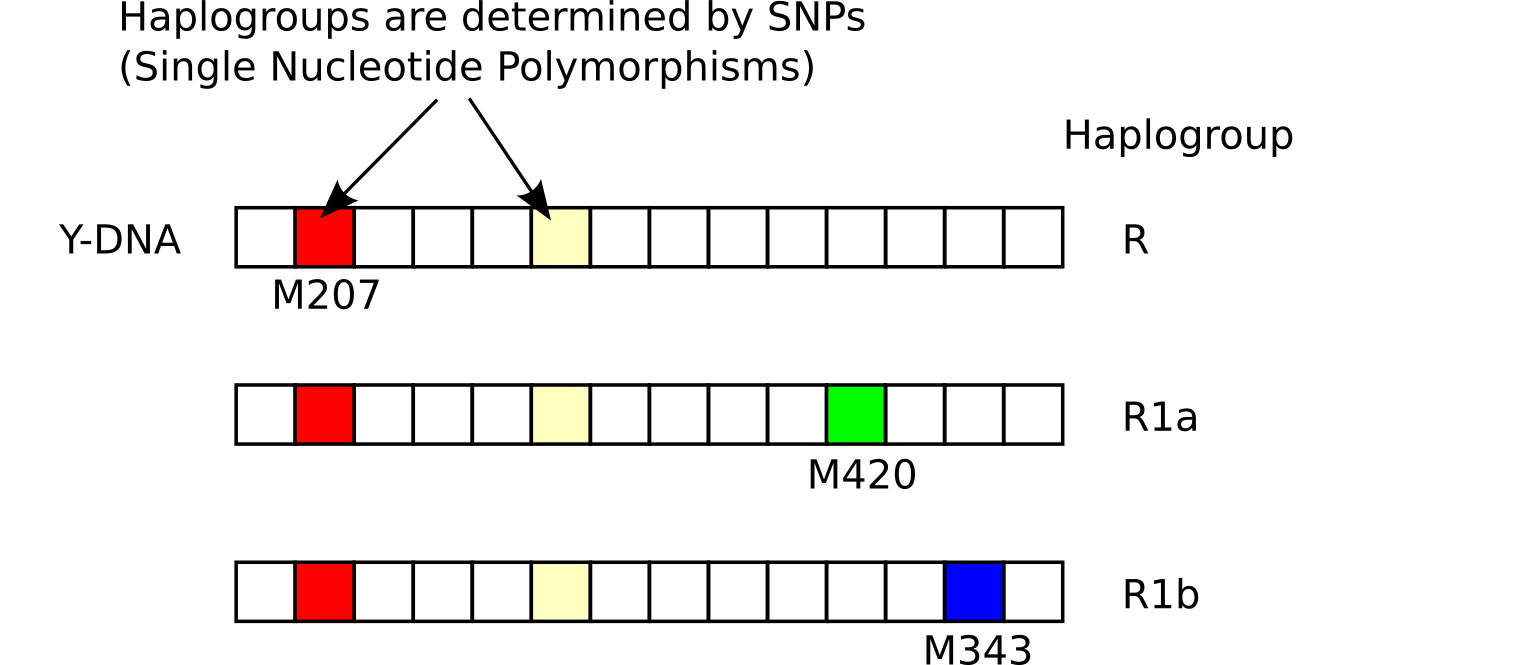
\includegraphics[width=13cm]{img/haplogroups.png}
\caption{\label{haplogroup} A set of single mutations
defines a person's haplogroup. Persons who belong to the
same haplogroup usually share a common ancestor within a
few thousand years.}
\end{figure}

Figure \ref{haplogroup} illustrates a typical situation.
Many Europeans belong to haplogroup R, which is characterized
by the mutation M207 and others which are not mentioned here.
The M207 marker is inherited throughout all following ancestral
lines. Later the mutations M420 and M343 occurred. They are
mutually exclusive to each other thus defining separate
lineages. The marker M420 defines the haplogroup R1a which
is common in Eastern Europe and the marker M343 defines the
haplogroup R1b which is common in Western Europe. Because
all people who belong to R1a and R1b share the M207 marker
we know that they also share a common ancestor a long time
ago.

SNPs do not occur very often. Persons who belong to the
same haplogroup usually share a common ancestor within a
few thousand years. If you know your haplogroup it will
tell you something about your deep history (thousands
of years).


\subsection{Haplotypes}

Most people want to know more about family relationships.
Luckily there is another type of mutations that occurs much
more often than SNPs. This is the repetition of certain
genetic patterns. They are called STRs (Short Tandem Repeats)
and group people into haplotypes.

\begin{figure}[ht]
\centering
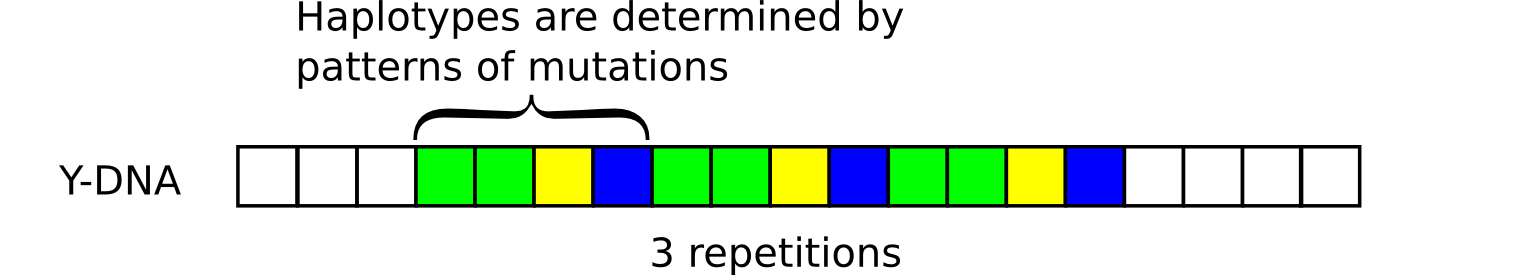
\includegraphics[width=13cm]{img/haplotypes.png}
\caption{\label{haplotype} A person's haplotype is defined
by patterns of mutations. Persons with the same haplotype
usually share a common ancestor within a few hundred years
if they take a standard test with 37 markers or more.}
\end{figure}

On the Y chromosome there are many different patterns that
repeat themselves. Every pattern has a name, for example DYS393.
If we count the number of repetitions for a specific pattern
we get a value, for example DYS393=13. Figure \ref{haplotype}
illustrates the situation for an exemplary marker. The pattern
is repeated 3 times. So this marker has a value of 3.

If a mutation occurs the number of repetitions changes. A 
single marker mutates rarely but the modern standard tests
use many markers at the same time, most often 37, 67 or
111. The combination of all these markers defines
a haplotype. Persons who share the same haplotype usually
also share a common ancestor within a few hundred years.

It is important to realize that haplotypes are not as good
as haplogroups. Haplotypes sometimes overlap between separate
lineages. So when working with haplotypes the haplogroup
should also be known.

Phylofriend uses haplotypes to calculate genetic distances
between persons by counting the number of different mutations.


\subsection{Phylogenetic Trees}

Phylogenetic trees group people together according to their
genetic distances. They give us a picture of how different
persons are related.

\begin{figure}[ht]
\centering
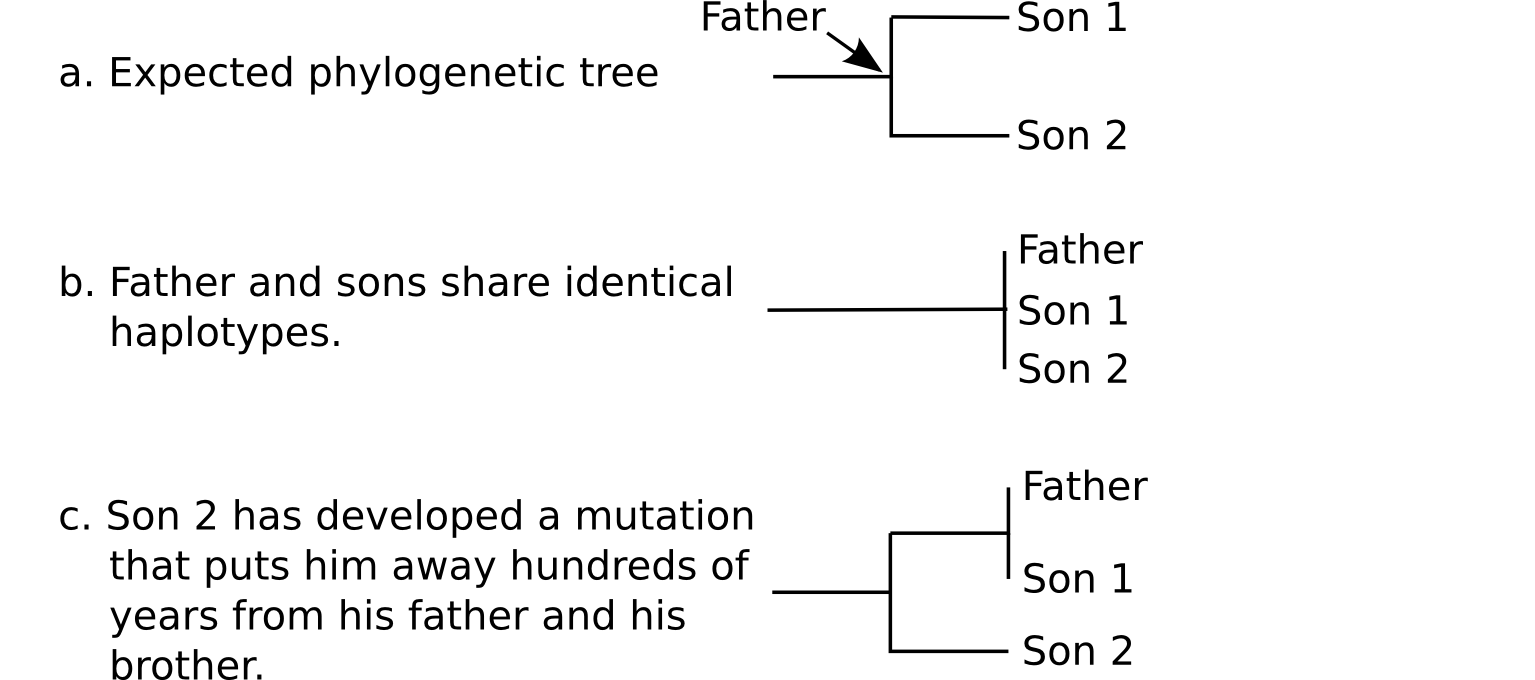
\includegraphics[width=13cm]{img/phylotrees.png}
\caption{\label{phylotrees} Phylogenetic trees group persons
together according to their genetic distances. Genetic
distances are often associated with time scales but this
is only true for long time spans.}
\end{figure}

Figure \ref{phylotrees} shows some exemplary trees. If a
father has two sons we would expect that both sons are at
a little genetic distance away from their father. If they
are not twins they also should be separated by each other.
Tree a illustrates this situation. This is exactly the
tree we would get if we could measure the genetic distance
at a high resolution and know the birth dates of father and
sons. Because we know the birth dates we would put the father
before the sons and associate the horizontal axis with a
time scale assuming that genetic distance is proportional
to time.

Reality however shows a different picture. The currently
available standard tests (37, 67 and 111 markers) only offer
a low resolution. So most often we can not measure any genetic
distance between father and sons. This is illustrated by
tree b. Because the tree illustrates genetic distances and
not time distances father and sons are all side by side.

If son 2 develops a mutation by chance we get a confusing picture.
Son 2 is suddenly far away from his father and his brother.
This is shown by tree c. The reason for the great distance
between father and son 2 is the low resolution of the test.
If we take the mutation rates from \cite{Kly12} we can
calculate how long it takes on average for a mutation to
occur. For a 37 marker test the result is 280 years, for
a 67 marker test 210 years and for a 111 marker test 130
years. 

This means if the father and his sons took a 37 marker test
and son 2 has developed a mutation by chance he will appear
to be 280 years away from his father but the only reason for
that is the low resolution of the test.

In most cases the standard tests are good enough. We do not
need a paternity test for genealogical purposes but it is
important to remember that the standard tests only places
persons into time frames of hundreds of years.


\subsection{Genetic Distance}

There are many ways to calculate genetic distances. Here we
use the method of mutation counting as described by Anatole
Klyosov in \cite{Kly09}.
We just count the number of mutation one persons differs from
another and take the result as the genetic distance.
Take a look at these two 6-marker haplotypes:

\vspace{1em}
\begin{tabular}{lrrrrrr}
       & DYS393 & DYS390      & DYS19 & DYS391      & DYS385a & DYS385b \\
Carl   &     13 & 24          & 14    & 11          & 11      & 14 \\
Clas   &     13 & \textbf{23} & 14    & \textbf{12} & 11      & 14
\end{tabular}
\vspace{1em}

At DYS390 and DYS391 Clas differs from Carl by one mutation.
Thus their genetic distance on the 6-marker scale is 2.

To represent this genetic distance in years we need to know
how often mutations occur. Thus we need a mutation rate.
The mutation rate is defined as follows:

\begin{equation}
k = \frac{m}{g y} \label{mutationrate}
\end{equation}

\begin{tabular}{ll}
k: &  Mutation rate per marker and generation\\
m: &  Number of mutations \\
g: &  Number of generations \\
y: &  Number of Y-STR values (markers)
\end{tabular}
\vspace{1em}

Mutation rates are derived from sample populations. But
mutations occur by coincidence. Thus for a precise measurement
we need large numbers of mutations. Different family lineages
often expose different mutation rates. So the standard mutation
rates should be considered as a first estimate. You can use
Phylofriend's \emph{cal} option to adjust your data to
historic events.

Now we can use equation \ref{mutationrate} to calculate a
genetic distance in generations. Formula \ref{mutationrate}
is equivalent to:

\begin{equation}
g = \frac{m}{k y} \label{generationdistance}
\end{equation}

This gives us the number of generations between Carl and Clas.
The only thing we still need to know is the generation time.
For historical purposes a generation time of 25 years is
commonly used. We get the time by multiplying the number
of generations with the generation time.

\begin{equation}
t = g d           \label{generationtime}
\end{equation}

\begin{tabular}{ll}
t: &  Genetic distance in years\\
g: &  Number of generations \\
d: &  Generation time in years
\end{tabular}
\vspace{1em}

By substituting $g$ with formula \ref{generationdistance}
we get the genetic distance in years:

\begin{equation}
t = \frac{m d}{k y} \label{timedistance}
\end{equation}

\begin{tabular}{ll}
t: &  Genetic distance in years\\
m: &  Number of mutations \\
d: &  Generation time in years\\
k: &  Mutation rate per marker and generation\\
y: &  Number of Y-STR values (markers)
\end{tabular}
\vspace{1em}

Let us try this out. The number of mutations between Clas
and Carl is 2. The mutation rate for a 6-marker haplotype
is 0.002 \cite{Kly09}. So

\begin{equation}
t = \frac{2 \cdot 25}{0.002 \cdot 6} = 4167\ years
\end{equation}

Wow, that is a very long time. But what does this number
actually mean? First, it is an average value and there is
a very big margin of error to it but it is useful as a first
estimate and to group people together according to their
genetic distance. Second it is the time Clas and Carl would
be separated if Clas would be an ancestor of Carl (or the
other way round). It is not the time to their most recent
common ancestor (TMRCA).

If Clas and Carl would be living today, how long would be the
the time to their most recent common ancestor? The first guess
is that the common ancestor would be in-between his descendants
in terms of genetic distance. So Claus and Carl would be
$4167years / 2 = 2085years$ away from him. 

This is a good first guess but unfortunately reality is much
more complicated. Mutations occur by coincidence and due to
the laws of statistics some people develop only a few mutations
while others develop much of them. So our first guess may give
a totally wrong impression. Generally it is not a good idea to
calculate the time to a common ancestor just based on the results
of two people. The best way is to identify a group of people who
share a common lineage and calculate the time to the most recent
common ancestor for the whole group. Anatole Klyosov describes
how this is done in \cite{Kly09}.

For those who still want to use a TMRCA value based on the results
of just two people Bruce Walsh has developed a method to give
a time estimate\cite{Wal01}. This is better than the naive
calculation we have used before but it is still an estimate and
it is only valid for demographically stable populations.

The whole story is of course more complicated than the simple
calculation presented here. Different mutation models exist
and some genetic markers should be treated in a special way.
Phylofriend uses a hybrid mutation model that is a mixture
of the stepwise mutation model and the infinite alleles model.
Both models are explained by Bruce Walsh in \cite{Wal02}.


\subsection{Modal Haplotype}

If we have a group of people we are interested in the
haplotype of their most recent common ancestor. This is
called the modal haplotype, base haplotype or ancestral
haplotype. The following table shows the haplotypes of three
persons on the 6-marker scale and their modal haplotype.

\vspace{1em}
\begin{tabular}{lrrrrrr} \label{tblmodalhaplotype}
       & DYS393 & DYS390      & DYS19       & DYS391      & DYS385a     & DYS385b \\
modal  &     13 & 24          & 14          & 11          & 11          & 14 \\
Peter  &     13 & 24          & \textbf{15} & 11          & 11          & 14 \\
Carl   &     13 & 24          & 14          & 11          & \textbf{12} & 14 \\
Clas   &     13 & \textbf{23} & 14          & \textbf{12} & 11          & 14
\end{tabular}
\vspace{1em}

The modal haplotype can easily be calculated. If we use
equation \ref{timedistance} to calculate the genetic distance
in years for just a single marker we see that it takes 12500
years on average for a single marker to mutate only once. 
Thus for most practical purposes a single marker rarely mutates
at all. So for a single marker we just look which value occurs
most often and take this as the modal value.

Phylofriend uses this simplified approach. For many thousands
of years it is no longer valid. Calculating the median values
would be a better choice then. The problem with the median
approach is that some markers show rather big leaps when mutating.
This could lead to wrong results. I recommend that you always
take a good look at your data to see which method would be
appropriate.


\subsection{Age Calculation}

\subsubsection{Mutation Counting}

The simplest method to calculate the time to the most recent
common ancestor (TMRCA) for a group of people is mutation
counting as described in great detail by Anatole Klyosov in
\cite{Kly09}. Here a give a short overview only.

First we calculate the modal (ancestral) haplotype. Then we
count the mutations of every single group member relative to
the modal haplotype and take the average. This should be a
good estimate for the group's genetic distance to their ancestor. 

Again we use the definition of the mutationrate \ref{mutationrate}
but this time we use the average value:

\begin{equation}
k = \frac{\bar{m}}{g y} \label{averagemutationrate}
\end{equation}

\begin{tabular}{ll}
k: &  Mutation rate per marker and generation\\
$\bar{m}$: &  Average number of mutations relative to modal haplotype\\
g: &  Number of generations \\
y: &  Number of Y-STR values per haplotype
\end{tabular}
\vspace{1em}

As mutations occur by coincidence equation \ref{averagemutationrate}
is only valid for sufficiently high values of $\bar{m}$.
By using the definition of the average, equation
\ref{averagemutationrate} is equivalent to

\begin{equation}
k = \frac{\sum_{i=1}^{N} m_i}{N g y}
\end{equation}

or

\begin{equation}
g = \frac{\sum_{i=1}^{N} m_i}{N k y}\label{tmrcagenerations}
\end{equation}

\begin{tabular}{ll}
g: &  Number of generations \\
$m_i$: &  Number of mutations of haplotype i relative to modal haplotype\\
N: &  Number of haplotypes (persons) \\
k: &  Mutation rate per marker and generation\\
y: &  Number of Y-STR values per haplotype
\end{tabular}
\vspace{1em}

Equation \ref{tmrcagenerations} is the time to the most recent
common ancestor in generations. If we know the generation time
$d$ we can write this (see equation \ref{generationtime}) as

\begin{equation}
t = d \frac{\sum_{i=1}^{N} m_i}{N k y}
\end{equation}

\begin{tabular}{ll}
t: & Time to most recent common ancestor (TMRCA)\\
d: & Generation time\\
$m_i$: &  Number of mutations of haplotype i relative to modal haplotype\\
N: &  Number of haplotypes (persons) \\
k: &  Mutation rate per marker and generation\\
y: &  Number of Y-STR values per haplotype
\end{tabular}
\vspace{1em}

The following example shows how to use the formula but it
is intended as an easy to understand educational exercise.
For real world applications more haplotypes (rule of thumb:
use at least 5) and a bigger number of average mutations
(4 or more is quite good) is needed. 

The table on page \pageref{tblmodalhaplotype} contains three
haplotypes on the 6-marker scale ($N=3$, $y=6$). Peter and
Carl differ by one mutation to the modal haplotype and Clas
by two. We use a generation distance of 25 years ($d=25$)
and the average mutation rate on the 6-marker scale is
0.002\cite{Kly09}. So we get

\begin{equation}
t = 25 \cdot \frac{1 + 1 + 2}{3 \cdot 0.002 \cdot 6} = 2778\ years
\end{equation}

Of course the simple method of mutation counting comes not without
problems. The biggest one is the correct distribution of the
population sample. For example if you want to calculate the
TMRCA for a family which is just a few hundred years old
and add a person by accident who is at a distance of several
thousand years your TMRCA value will be much too large.

On the other hand if you want to calculate the age of a whole
haplogroup and add a large number of members from one family
who are all very close together your TMRCA value will be much
too small. So this method must be handled with care.

A more general problem is that mutation rates are derived
from population samples and there is no guarantee that they
fit to your data set. So whenever possible try to find some
historical event to calibrate your data.


\subsection{From Distances to Trees}

Phylofriend computes genetic distances between different
persons. These distances can be used to derive phylogenetic
trees using standard algorithms that are implemented by
the PHYLIP\cite{Phylip} program.

Genetic distances are often represented by two-dimensional
drawings that are easy to understand. Here we label the
distance components as \emph{Component 1} and 
\emph{Component 2}. Usually the values for each component
are derived from many markers by using principal component
analysis\cite{Shl09}.

\begin{figure}[ht]
\centering
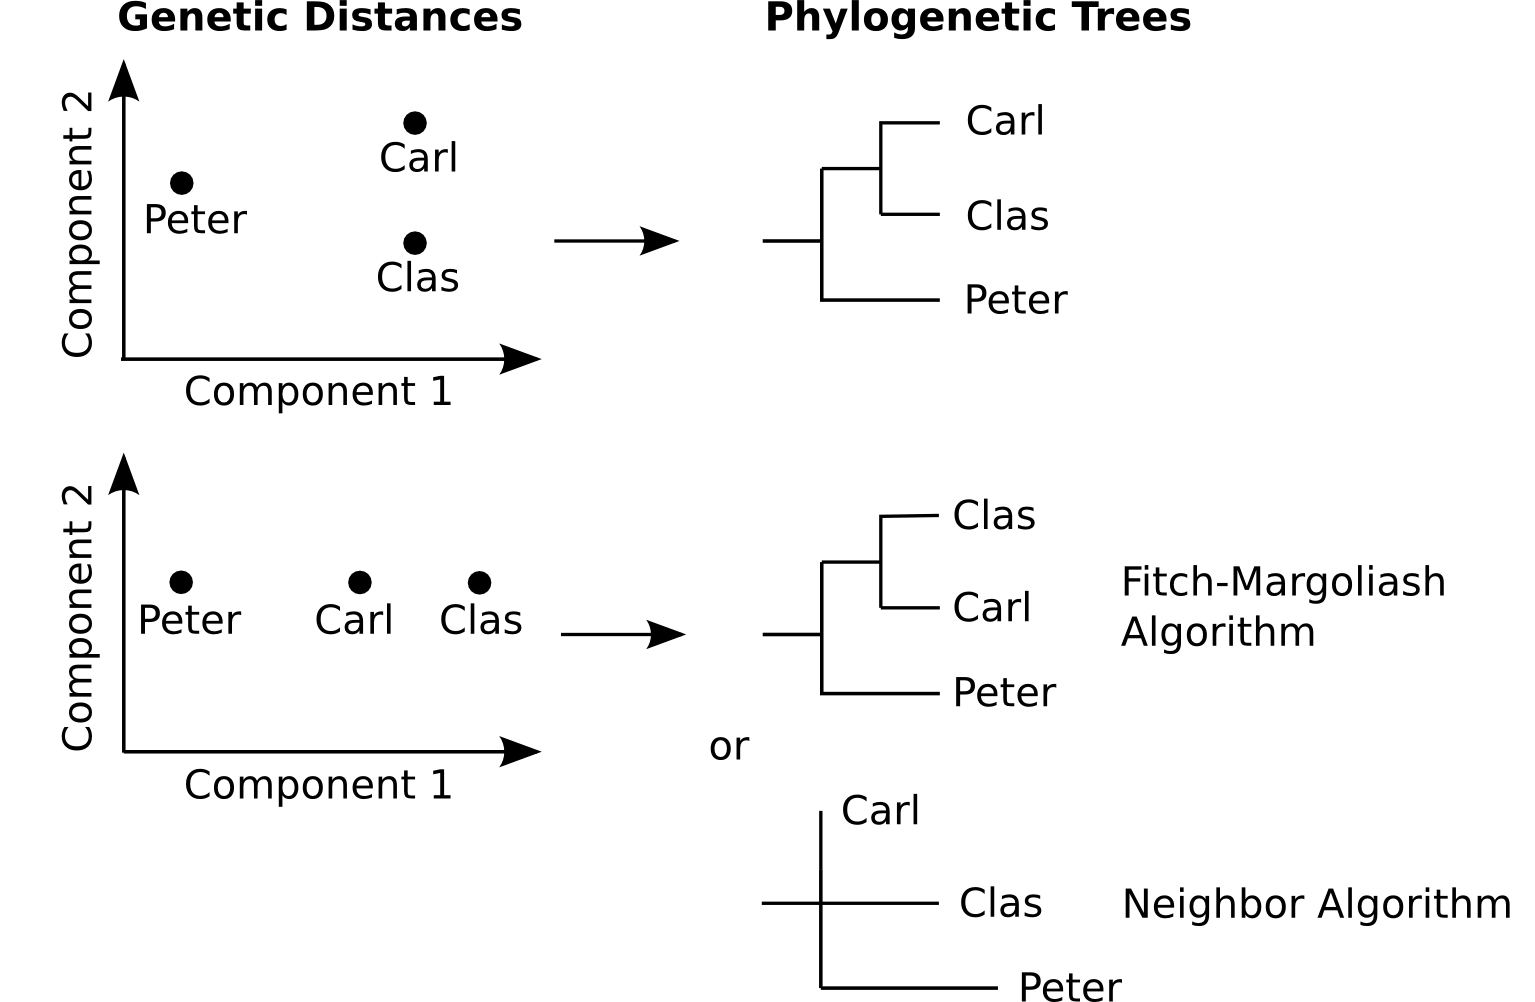
\includegraphics[width=13cm]{img/distancetrees.png}
\caption{\label{distancetrees} Genetic distances can be
represented by phylogenetic trees. Different algorithms
often yield different results.}
\end{figure}

Figure \ref{distancetrees} shows the genetic positions of
several persons and the corresponding phylogenetic trees.
In the first example Carl and Clas are close together. So
they are also grouped together in the tree. Peter is at a
longer distance but the distance to Carl and Clas is the
same. Thus he is put into a separate branch. The genetic
distance between the persons is represented by the length
of the horizontal lines in the tree.

The second example is slightly more complicated. Carl and
Clas are still close together but Peter is at a different
distance to each of them. The trees were constructed by
using two different methods, Fitch-Margoliash (kitch program)
and Neighbor. Fitch-Margoliash groups Carl and Clas together
and puts Peter at a medium distance from both of them. This
is a sensible approach because some people develop many
mutation and others develop less. So the ancestor of Carl and
Clas was probably somewere in-between. However the resulting
tree does not represent the genetic distances correctly but
it displays a very nice representation of temporal evolution.

The neighbor method tries to represent the genetic distances
as good as possible. In this case it is accurate but it gives
you a bad idea of temporal evolution.

For a high quality data set both methods should yield similar
results in grouping people together. The real problem is that
mutations occur by coincidence and we often have a very sparse
collection of descendants who are at large genetic distances
to each other.

\begin{figure}[ht]
\centering
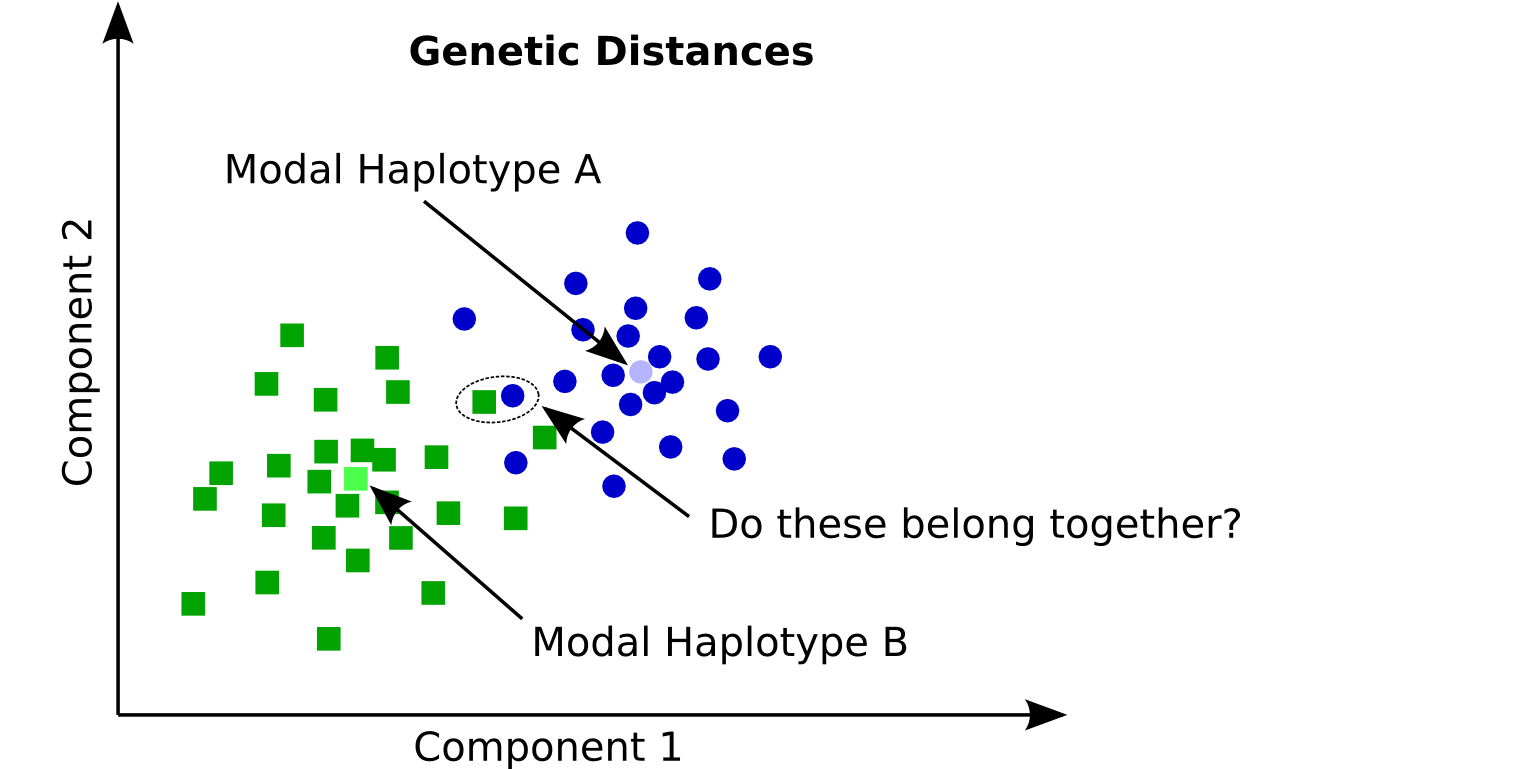
\includegraphics[width=13cm]{img/distances.png}
\caption{\label{distances} Haplotypes and genetic distances
of two families. Although both lineages have a different modal
(ancestral) haplotype the haplotypes of individuals from
both families are sometimes close together. In such cases
phylogenetic tree algorithms yield wrong results.}
\end{figure}

Figure \ref{distances} shows a more realistic situation.
It represents the genetic positions of members from two
different families. All members of one family descent from
one common ancestor. Due to the laws of statistics most
family members are close to his haplotype. So it can be
calculated. It is called the ancestral or modal haplotype.

Other family member are at a greater distance from the
ancestor. Sometimes members from different families come
close to each other. In such cases all algorithms will 
give you wrong results.

This is the reason why it is so important to test for
haplogroups before creating a phylogenetic tree. Haplogroups
are caused by very stable mutations. Haplotypes often overlap.
So it should be ensured that all persons in a tree belong
to the same haplogroup.




















